\documentclass[a4paper,10pt]{article}
\usepackage{graphicx}
\usepackage{verbatim}
% \usepackage{lstlisting}
\usepackage{subfig}
\usepackage{float}
 \usepackage[spanish]{babel}   %ver bien como es
\usepackage[utf8]{inputenc}


\begin{document}

\tableofcontents

\newpage


\begin{center}
\section*{Aclaraciones Generales}
\addcontentsline{toc}{section}{Aclaraciones Generales} 

\begin{itemize}
\item La implementación de todos los algoritmos se realizó en lenguaje C++.

\item Para calcular los tiempos de ejecución de los algoritmos se utilizó la función gettimeofday(), que se encuentra en la librería $<sys/time.h>$. Dado que dicha función funciona solamente en sistemas operativos de tipo linux, se debe compilar con el flag -DTIEMPOS en este tipo de sistemas para poder hacer uso de las mismas.

\item Para la realización de los gráficos se utilizó Qtiplot
\end{itemize}

\end{center}

\newpage

\section*{Introducci\'on}
\addcontentsline{toc}{section}{Introducci\'on}

En el presente trabajo se realizaron diferentes aproximaciones a la resoluci\'on del problema de optimizaci\'on MAX-SAT. Dicho problema proviene del problema de decisi\'on SAT. 

El problema SAT se basa es decidir si un conjunto de cl\'ausulas en forma normal conjuntiva, tiene alguna asignaci\'on de las variables que las componenen, tal que la evaluaci\'on de todas las clasulas sea verdadera con dicha asignaci\'on. \'Este es un problema muy importante dentro del campo de la teor\'ia de la complejidad, esto se debe a que SAT fue el primero que se identific\'o como NP-Completo. El Teorema de Cook demuestra que el algoritmo SAT pertenece a esta clase de algoritmos.

La importancia de este algoritmo no radica solamente en haber sido el primero en ser caracterizado como NP-Completo, se demostr\'o que el problema SAT puede ser reducido al problema 3-SAT, que es basicamente el mismo problema pero en el cual todas las cl\'ausulas tienen un m\'aximo de 3 literales. Adem\'as de probar la reducci\'on, se demostro que este problema tambi\'en pertenece a la clase NP-Completo (A diferencia del problema 2-SAT, para el cual se conoce un algoritmo polinomial para resolverlo). Esta reducci\'on del problema a 3-SAT es un resultado importante, ya que luego para probar que otros problemas se encuentran tambi\'en en esta clase, se utilizaron reducciones a 3-SAT mostrando la equivalencia en cuanto a la complejidad de resoluci\'on.

\section*{Situaciones de la vida real que se pueden modelar utilizando MAX-SAT}
\addcontentsline{toc}{section}{Situaciones de la vida real que se pueden modelar utilizando MAX-SAT} 

El problema de max-sat tiene varias aplicaciones pr\'acticas. Muchas de ellas aplicadas a la biolog\'ia y otros campos cient\'ificos. Sin embargo, el problema de max-sat puede aplicarse a situaciones cotidianas.

El problema de max-sat se puede aplicar cuando tenemos alguna entidad que esta satifescha si se cumple algo que pide, o si por lo menos no se cumple una de las cosas que pide que no se cumpla.

Supongamos una c\'amara de diputados donde hay varios proyectos de ley. Cada legislador tiene una opini\'on formada sobre los proyectos de ley, pero podr\'ia ser que sobre algunos proyectos no est\'e ni a favor ni en contra. Adem\'as tambi\'en supongamos que es una \'epoca complicada para los partidos pol\'iticos ya que ninguno logra erigirse con firmeza. Es por esto que los legisladores son bastante permisivos y se contentan de varias maneras. Si se aprueba alg\'un proyecto de ley que ellos apoyan, est\'an satisfechos porque pueden volver a su partido y decir que ese proyecto de ley se aprob\'o gracias a la presi\'on que ellos ejercieron. Por otro lado, los legisladores tambi\'en quedan satisfechos si alg\'un proyecto que no estaban a favor no se aprueba, porque de esta manera pueden decir que frenaron un proyecto de la oposici\'on gracias a la presi\'on que ellos ejercieron. De esta manera, este problema se puede modelar mediante max-sat donde cada clausula es un diputado y cada variable es un proyecto de ley diferente. De esta manera, la c\'amara de senadores puede, resolviendo max-sat, saber que leyes aprobar y cuales no para contentar a la mayor cantidad de diputados y que la situaci\'on p\'olitica del pa\'is pase a una peor situaci\'on.


En este ejemplo se puede aplicar max-sat, pero en realidad es solo un caso particular de lo explicado al principio. Es decir, en vez de ser legisladores podr\'ian ser otras personas u otras cosas que pidan requisitos sobre otras cosas, pero lo importante es que se satisfacen si alguna cosa de la que piden se hace verdadera, o alguna cosa de la que piden como falsa se haga falsa.


\bigskip

Otras situaciones diferentes donde se puede aplicar max-sat y donde las entidades no tienen que ser tan laxos como lo eran los anteriores diputados, podr\'ia ser una situaci\'on donde las entidades pidan muchas cosas a favor y pidan una sola en contra. Por ejemplo, podr\'iamos tener una familia que se va de vacaciones, dicha familia tiene 3 hijos. 

Un hijo le gustar\'ia ir a la playa o tambi\'en quedarse en su casa e ir a una colonia, pero no le gusta para nada la idea de ir a pasar sus vacaciones en la monta\~{n}a.

El segundo hijo le gusta mucho hacer actividades fis\'icas por lo que esta a favor de ir a la colonia y hacer deportes, o ir a la monta\~{n}a para hacer caminatas, pero jamas ir\'ia a la playa porque piensa que es solo ir a tirarse a tomar sol. 

En \'ultimo lugar, el tercer hijo piensa igual que el segundo porque \'este lo ha sobornado.

Luego, los padres tienen que resolver este problema max-sat donde las clausulas son sus hijos y las variables son las vacaciones posibles. Cabe destacar que las vacaciones las pueden dividir por semanas y pasarlas en m\'as de un lugar. Si bien en esta familia los hijos y las diferencias son pocas, en una familia numerosa, esto podr\'ia generar una gran pelea familiar que se resolver\'ia con max-sat.


\section*{Algoritmo exacto para MAX-SAT}
\addcontentsline{toc}{section}{Algoritmo exacto para MAX-SAT} 
Como su nombre lo indica, el algoritmo exacto para Max-Sat se encarga de resolver el problema exactamente, es decir, que el resultado que retorna es la resoluci\'on que valida la mayor cantidad de cl\'ausulas posibles. Dado que no se conoce ning\'un algoritmo polinomial para resolver este problema, se implementaron 2 algoritmos de complejidad exponencial. Por un lado se implement\'o un algoritmo de fuerza bruta de simple implementaci\'on pero de muy baja eficacia en cuanto a tiempo de ejecuci\'on. Por otro lado, se implement\'o un algoritmo exacto mediante backtracking para poder evitar visitar todas las asignaciones de las variables posibles.

\subsection*{Algoritmo de fuerza bruta}
\addcontentsline{toc}{subsection}{Algoritmo de fuerza bruta}
En este algoritmo la idea es muy simple, se generan absolutamente todas las asignaciones posibles que existen, siendo estas $2^{v}$ donde v es la cantidad de variables. Luego, por cada una de las asignaciones se verifica cuantas cl\'ausulas valida, en el momento que una asignaci\'on supera el m\'aximo de cl\'ausulas hasta el momento, se actualiza la cantidad de cl\'ausulas validadas, as\'i como cual es la asignaci\'on que gener\'o este m\'aximo.

La idea de este algoritmo es tener una resoluci\'on muy simple del problema, es claro que el tiempo de ejecuci\'on va a ser muy malo, ya que se revisan todas y cada una de las asignaciones posibles y estas crecen en orden exponencial en funci\'on de la cantidad de variables. Sin embargo, cabe destacar que el algoritmo provee una resoluci\'on exacta del problema y con baja probabilidad de errores dada la simpleza del mismo.

A continuaci\'on se presenta el pseudoc\'odigo del mismo:

\begin{verbatim}
maxSatExacto(Vector cl\'ausulas, int variables)
vector asignacion
int max := 0
inicializar asignacion todos en falso
Para i = 1 hasta 2^variables
    int sat := 0
    Para j = 1 hasta tamanio(cl\'ausulas)
       Si haceTrue(asignacion, cl\'ausulas[j])
          sat:= sat + 1
       fin si
    fin para
    si sat > max
        actualizar max
        actualizar asignacionMax
    fin si
    asignacion := siguiente(asignacion,i+1)
fin para
devolver asignacionMax, max
\end{verbatim}

Lo que muestra el pseudoc\'odigo anterior es como, por cada asignaci\'on posible, se mira cada clausula y si la funci\'on \emph{haceTrue} devuelve true, entonces se suma 1 a la cantidad de satisfechas por esa asignaci\'on. Por \'ultimo, se mira cual asignaci\'on es la que tiene m\'as cl\'ausulas satisfechas.

La funci\'on \emph{haceTrue} lo que hace es simplemente mirar toda la clausula pasada como par\'ametro y ver si alg\'un literal esta asignado como verdadera, cuando encuentra uno deja de buscar y devuelve True. En caso contrario, si llega hasta el final de la clausula, devuelve False. 

Por otro lado, la funci\'on \emph{siguiente} se encarga de modificar la asignaci\'on para probar con todas las posibles.

\subsection*{Algoritmo de backtracking}
\addcontentsline{toc}{subsection}{Algoritmo de backtracking}

Luego de implementar un algoritmo exacto por fuerza bruta, se busc\'o realizar un algoritmo tambi\'en exacto pero tratando de lograr un menor tiempo de ejecuci\'on. El algoritmo logrado utiliza la t\'ecnica de backtracking para lograr mejores resultados (en cuanto a tiempo de ejecuci\'on), si bien en la siguiente secci\'on se ver\'a que la complejidad temporal es la misma para ambos algoritmos exactos, la t\'ecnica de backtracking provee de herramientas para no tener que consultar necesariamente por cada una de las asignaciones posibles, es en estas podas que este algoritmo mejora los tiempos de ejecuci\'on del anterior.

\bigskip

La idea de este algoritmo es la siguiente: se genera un \'arbol de asignaciones, donde cada nivel del \'arbol i representa todas las asignaciones posibles desde la variable 1 hasta la variable i. Este \'arbol es binario dado que se arranca de la asignacion nula y de all\'i se abren dos caminos, asignarle False a la variable 1, o asignarle True. Luego, cada rama se va bifurcando sucesivamente por cada variable nueva. Como se puede ver, en el peor caso que es que tengamos que recorrer todo el \'arbol, la cantidad de asignaciones nuevamente esta dada por $2^{v}$ al igual que en el algoritmo de fuerza bruta.

Una vez que se tiene el \'arbol de backtracking lo que se hace es comenzar a recorrerlo en alguna direcci\'on determinada. Cabe destacar que en el algoritmo implementado siempre se recorre primero la rama correspondiente a asignar falso a la variable y luego la otra.

La mejora del algoritmo radica en no recorrer todas las ramas posibles, esto se realiza de la siguiente manera: Al haber recorrido la primer rama del \'arbol llegando hasta una hoja, ya se tiene una mejor soluci\'on posible. Luego, cuando se este explorando una rama, lo que se hace es fijarse si esa rama ya posee m\'as cl\'ausulas insatisfechas que la mejor soluci\'on hasta el momento. En caso afirmativo, la rama ya no sirve ya que no se podra mejorar la soluci\'on y entonces se puede descartar todo el sub\'arbol que pende de esa rama. Posteriormente, se realiza el backtracking para ir por otro camino posible. 

Las principales diferencias con el algoritmo de fuerza bruta son:
\begin{itemize}
\item La implementaci\'on es bastante m\'as complicada ya que como se realiza backtracking, se debe guardar los estados intermedios de toda la rama que se esta analizando para poder volver hacia atras y tomar un nuevo camino. En el algoritmo de fuerza bruta, cada asignacion se contrasta con las cl\'ausulas originales por lo que solo se deben guardar una vez todas las cl\'ausulas.
\item El tiempo de ejecuci\'on deber\'ia ser menor en la mayor\'ia de los casos. Si bien el peor caso no cambiar\'ia es importante destacar que las podas realizadas pueden traer grandes beneficios en cuanto al tiempo de ejecuci\'on. Si, por ejemplo, ya se tuviese una soluci\'on donde n cl\'ausulas son insatisfechas y al asignar True a la variable 1, n+1 cl\'ausulas se vuelven insatisfacibles entonces se podr\'ia podar toda una mitad del arbol.
\item El algoritmo de fuerza bruta no puede ser influenciado por alguna heur\'istica, mientras que el algoritmo con backtraking s\'i. Lo que se quiere notar con esto, es que por m\'as que ya se tenga una soluci\'on con n cl\'ausulas insatisfechas, el algoritmo por fuerza bruta tiene que probar todas las asignaciones posibles; mientras que el algoritmo de backtracking ya puede comenzar podando ramas que tengan m\'as de n cl\'ausulas insatisfechas.
\end{itemize}


\subsection*{Complejidad de algoritmos exactos}
\addcontentsline{toc}{subsection}{Complejidad de algoritmos exactos}

En primer lugar, se analizar\'a la complejidad del algoritmo realizado por fuerza bruta.

El mismo presenta un ciclo que se realiza $2^{v}$ veces, dado que esa es la cantidad total de asignaciones diferentes, siendo v la cantidad de variables. Una vez dentro de este ciclo, encontramos otro ciclo que itera sobre la totalidad de las cl\'ausulas, haciendo que este ciclo se realice c veces. 

Luego, dentro de este ciclo se llama a la funcion haceTrue. Esta funci\'on lo que hace es fijarse en todos los literales de la clausula si se encuentra asignado como verdadero. Dado que el hecho de fijarse es O(1), ya que es mirar un array, y dado que la clausula como mucho tiene 2*v literales (todas las variables negadas y sin negar), se puede ver que esta funci\'on es O(v).

Por \'ultimo, las otras operaciones que se realizan dentro del ciclo principal tienen menor complejidad que lo mostrado anteriormente, ya que son asignaciones que toman O(1) o es la funci\'on siguiente que toma O(v).

Por lo mostrado anteriormente resulta que la complejidad temporal del algoritmo es O($(2^{v})$*c*v)
Como se puede ver, lo importante m\'as alla de la complejidad exacta, es que este algoritmo es exponencial en funci\'on de la cantidad de variables. Cabe destacar que si bien se podri\'an encontrar algoritmos con mejor complejidad, esta no podr\'ia ser menor que exponencial en el caso que se quieran revisar todas las asignaciones posibles.

\bigskip

Complejidad del algoritmo exacto con backtracking:

Para realizar el c\'alculo de complejidad de este algoritmo tomaremos el peor caso posible. El mismo consiste en que ninguna rama sea podada y por lo tanto se tengan que revisar todos los nodos posibles del \'arbol. En este caso el ciclo principal que itera sobre todas las asignaciones posibles ser\'ia O($2^{v}$), ya que este es el orden de la cantidad de nodos del \'arbol. 

Luego, hay que analizar cuales son las operaciones que se realizan cada vez que el algoritmo se encuentra en un nuevo nodo. En primer lugar, se llama a la funci\'on resolver, la misma tiene un funcionamiento an\'alogo al explicado en el algoritmo por fuerza bruta; se fija en cada clausula si la misma se hizo verdadera, y cuenta las insatisfacibles, por lo que esta funci\'on toma O(c*v) operaciones. Luego, lo que se hace es copiar todo el estado al siguiente nodo para que se pueda procesar, al realizar esto se copian varios par\'ametros. Sin embargo, el orden temporal de esta copia esta dado por el orden que toma copiar todas las clasulas, dado que los dem\'as par\'ametros que se copian tienen menor orden espacial, ya que son solamente vectores. Cabe destacar que al copiar al siguiente nodo, s\'olo se copian las cl\'ausulas que no fueron satisfechas todav\'ia, ya que las dem\'as ya estan fuera del an\'alisis.

Se puede ver que copiar todo el estado toma O(c*v) operaciones ya que lo que se hace es copiar absolutamente todas las cl\'ausulas en el peor caso, donde cada una pueda tener hasta 2*v literales por lo justificado anteriormente.

Por \'ultimo, resumiendo lo anteriormente explicado se puede ver que cuando se revisa un nodo toma O(c*v) operaciones, y en el peor caso hay que revisar O($2^{v}$) nodos; por lo que la complejidad total de este algoritmo es O($(2^{v})$*c*v).

Como se puede ver, la complejidad del algoritmo de backtracking no es mejor que el algoritmo exacto por fuerza bruta, sigue siendo exponencial. De hecho, se puede notar que en el peor caso posible, el algoritmo de backtracking es m\'as lento que el algoritmo por fuerza bruta dado el overhead que produce copiar todo el estado al siguiente nodo del \'arbol para que se pueda seguir procesando.

Sin embargo, en la mayor\'ia de los casos, el algoritmo con backtracking presenta resultados temporalmente mejores que el algoritmo de fuerza bruta, ya que se podan varias ramas haciendo que no se tenga que visitar todas las asignaciones posibles.

\medskip

Cabe destacar que la ventaja temporal que gana el algoritmo de backtracking, genera una mayor complejidad espacial ya que en todo momento se debe tener todos los estados de los nodos de la rama que se esta visitando para poder caminar hacia atras. Luego la complejidad espacial del algoritmo de fuerza bruta es O(c*v) ya que se guardan una vez todas las cl\'ausulas, mientras que la complejidad espacial del algoritmo de backtracking es O(c*v*v) ya que, en el peor caso, se guardan todas las cl\'ausulas una vez por cada nodo de la rama que se esta analizando, que a lo sumo tiene v nodos.




\section*{Heur\'istica constructiva para MAX-SAT}
\addcontentsline{toc}{section}{Heur\'istica constructiva para MAX-SAT} 
En esta secci\'on se explicar\'a el uso de una heur\'istica constructiva para resolver el problema.

La motivaci\'on principal de utilizar diferentes heur\'isticas para resolver el problema de Max-Sat es que, como se vio en la secci\'on anterior, los algoritmos exactos conocidos son de orden exponencial por lo que solo se pueden correr con instancias relativamente peque\~{n}as.

La idea entonces es realizar un algoritmo que no sea exacto, sino que arroje una soluci\'on aproximada, pero en un tiempo polinomial para poder correr instancias m\'as grandes.

En esta primer aproximaci\'on, se realiz\'o una heur\'istica constructiva, esto quiere decir que se va construyendo una soluci\'on mediante alg\'un criterio que se supone (y luego se ver\'a que se puede demostrar) que es adecuado para obtener un buen resultado.

En este caso, la heur\'istica constructiva seguir\'a una estrategia golosa para ir armando la soluci\'on. Lo que hace esta heur\'istica es revisar todas las cl\'ausulas buscando cual es el literal que m\'as se repite. Una vez encontrado dicho literal lo que se hace es asignar True a este literal y actualizar las cl\'ausulas en base a esta asignaci\'on.

Actualizar las cl\'ausulas consiste en dos tareas, en primer lugar se borran todas las cl\'ausulas que contenian este literal ya que ya fueron satisfechas mediante la asignaci\'on y se actualiza el contador de cl\'ausulas satisfechas. Por otro lado, en las cl\'ausulas restantes, se borra el literal negado ya que este no sirve para futuras elecciones porque al asignar True al literal elegido, el literal negado tendra necesariamente valor falso.

Luego de realizar esta actualizaci\'on, se continua iterativamente con esta estrategia golosa hasta encontrar una asignaci\'on completa de las variables.

A continuaci\'on se muestra el pseudoc\'odigo de la heur\'istica constructiva:

\begin{verbatim}
Constructiva(Vector cl\'ausulas, int V)
Max := 0
Comenzar con asignacion vacia
mientras asignacion no este completa
      Tomar literal l que mas se repita
      Asignar True a l
      Para i de 1 hasta tamanio(cl\'ausulas)
         Si esta(l, clausula[i])
             borrar clausula[i]
             Max := Max + 1
         fin si
      fin para
      Para i de 1 hasta tamanio(cl\'ausulas)
         Si esta(-l, clausula[i])
             borrar(-l, clausula[i])
         fin si
      fin para
fin mientras
devolver asignacion y Max
\end{verbatim}

\subsection*{Aproximaci\'on del resultado}
\addcontentsline{toc}{subsection}{Aproximaci\'on del resultado}

Es importante destacar que a priori esta heur\'istica podr\'ia arrojar resultados que no se acercasen al verdadero valor del problema. La heur\'istica parece razonable ya que siempre se elige el literal que m\'as cl\'ausulas satisface, y luego se va iterando hasta que no queden m\'as variables para asignar. Tambi\'en es importante destacar que, si bien la heur\'istica parece razonable se puede encontrar r\'apidamente casos en los cuales \'esta aproximaci\'on golosa no nos devuelva el resultado exacto. Dada estas observaciones, se busc\'o encontrar algun tipo de cota para el resultado entregado por la heur\'istica, en funci\'on del verdadero resultado.

Dada esta heur\'istica golosa, se puede ver que en realidad se trata de un algoritmo aproximado. Si se denota $c_{max}$ como la cantidad m\'axima de cl\'ausulas satisfacibles, $c_h$ al resultado entregado por la heur\'istica y m al m\'inimo n\'umero de literales contenido en cualquiera de las cl\'ausulas, se cumple que\footnote{Cita Bibliogr\'afica 1}:


\begin{equation}
c_h \geq \frac{m}{m+1}*c_{max}
\end{equation}

Dada la ecuaci\'on anterior, se tiene una cota para el resultado que depende del m\'inimo n\'umero de literales en cualquier cl\'ausula. Cabe destacar que en la implementaci\'on de esta heur\'istica, y en los casos de prueba utilizados, no se hace ninguna menci\'on particular a la cantidad m\'inima de literales de las cl\'ausulas. En este caso, podemos acotar por el peor caso que ser\'ia tener cl\'ausulas de un solo literal.

En dicho caso, la heur\'istica utilizada ser\'ia un algoritmo $\frac{1}{2}$-aproximado, es decir que el resultado arrojado jam\'as se encontrar\'a por debajo de la mitad del valor real del problema. En el caso de que el m\'inimo n\'umero de cl\'ausulas suba (lo que suele pasar en la pr\'actica), la cota tambi\'en se ajustar\'a dando una mejor aproximaci\'on.

\subsection*{Complejidad de la heur\'istica constructiva}
\addcontentsline{toc}{subsection}{Complejidad de la heur\'istica constructiva}

La heurística elige de manera golosa el literal que más cl\'ausulas satisface y lo hace verdadero. Esto se repite hasta que la asignación de las variables esté completa.

Para elegir el literal que más cl\'ausulas satisface se mantiene, por cada literal, un conjunto con las cl\'ausulas que haría verdaderas y que todavía no están satisfechas.

Al realizar cada elección se debe actualizar la estructura, eliminando cada una de las cláusulas satisfechas de los conjuntos en los que aparezcan. Como se tiene un conjunto por cada literal, se van a borrar las cláusulas satisfechas de $v$ conjuntos, donde $v$ es la cantidad de variables del problema. En el algoritmo se van a satisfacer a lo sumo $c$ cláusulas. Por lo tanto a cada cláusula satisfecha se la va a borrar de $v$ conjuntos, teniendo el borrado una complejidad en $O\left( log \left( c \right) \right)$, donde $c$ es la cantidad de cláusulas del problema. Por lo tanto, mantener la estructura va a tener una complejidad en $O\left( c \times v \times log \left( c \right) \right)$.

El conjunto utilizado para guardar las cl\'ausulas que haría verdaderas un literal está implementado en una estructura de árbol que garantiza inserción y borrado en $O\left( log \left( e \right) \right)$, donde $e$ es la cantidad de elementos del conjunto.

Como se tiene que recorrer todas las variables en cada asignación para mantener la estructura, se puede llevar un registro de cuál es el literal que más cláusulas, entre las aún insatisfechas, haría verdaderas. 

Luego, por todo lo explicado anteriormente, la complejidad temporal de la heur\'istica constructiva es $O\left( c \times v \ times log \left( c \right) \right)$.



\section*{Heur\'istica de b\'usqueda local para MAX-SAT}
\addcontentsline{toc}{section}{Heur\'istica de b\'usqueda local para MAX-SAT} 

La segunda he\'uristica implementada fue la de b\'usqueda local. Como su nombre lo indica, lo que hace esta heur\'istica es pararse sobre una soluci\'on y buscar localmente si se puede mover a otra soluci\'on \emph{cercana} con m\'as cl\'ausulas satisfechas. Dada la explicaci\'on anterior, se desprende que entonces se debe definir que significa que dos soluciones cercanas. Teniendo una asignaci\'on posible, se define una vecindad de asignaciones mediante alg\'un criterio que ser\'an las asignaciones \emph{cercanas} mencionadas anteriormente.

La idea principal de la heur\'istica es empezar con alguna asignaci\'on posible y luego buscar en la vecindad de esta soluci\'on si existe alguna asignaci\'on que satisfaga mayor cantidad de variables, si existe esta nueva asignaci\'on, entonces se cambia la asignaci\'on m\'axima actual por esta nueva y se vuelve a realizar una b\'usqueda local, ahora con la vecindad de la nueva asignaci\'on.

Esta heur\'istica finaliza cuando tenemos una asignaci\'on que es la mejor de todas entre ella y las asignaciones de su vecindad. Es decir, cuando se encuentra un m\'inimo local, la heur\'istica para y devuelve la mejor asignaci\'on encontrada hasta el momento.

Es importante destacar que la heur\'istica de b\'usqueda local necesita de una asignaci\'on inicial para comenzar a definir su vecindad y luego realizar la b\'usqueda. Como una primera aproximaci\'on se podr\'ia inicializar la heur\'istica con cualquier asignaci\'on, por ejemplo todas las variables en falso, el problema es que para caso de prueba diferente el espacio de asignaciones tiene una forma diferente. Esto puede llevar a que si inicializamos en cualquier asignaci\'on, se encuentre rapidamente un m\'aximo local que poco tenga que ver con la soluci\'on real del problema. 

La soluci\'on que se utiliz\'o para el problema explicado anteriormente es que la heur\'istica de b\'usqueda local sea inicializada con el resultado proviniente de aplicar la heur\'istica constructiva.

Es importante notar que la heur\'istica de b\'usqueda local no tiene permitido moverse a una asignaci\'on que satisfaga una menor cantidad de cl\'ausulas, por lo que se puede ver que el resultado arrojado por la b\'usqueda local es mejor o igual que el resultado de la heur\'istica constructiva en el caso de que se inicialice el procedimiento con el resultado de la heur\'istica constructiva.

De esta manera, reemplazando en la ecuaci\'on (1) (denotado $c_{local}$ al resultado de la b\'usqueda local):

\begin{equation}
c_{local} \geq c_{constr} \geq \frac{m}{m+1}*c_{max}
\end{equation}

Luego, dada la ecuaci\'on anterior y con una explicaci\'on an\'aloga a la propuesta en la heur\'istica constructiva, se puede ver que esta heur\'istica (inicializada de esta manera) tambi\'en se trata de un algoritmo $\frac{1}{2}$-aproximado y, de la misma manera, a medida que el m va subiendo, la cota va mejorando.

Cabe destacar que esta justificaci\'on es as\'i dado el hecho que en este trabajo en particular se utiliza la heur\'istica constructiva como punto de arranque para la b\'usqueda local. Sin embargo, en la bibliograf\'ia tambi\'en se encuentra demostrado que la b\'usqueda local cumple la misma cota sin necesidad de comenzar de ninguna asignaci\'on en particular\footnote{Ver cita bibliogr\'afica 1}.


\subsection*{Detalles de implementaci\'on}
\addcontentsline{toc}{subsection}{Detalles de implementaci\'on}

En primer lugar, es importante destacar como se definio la vecindad de una asignaci\'on, para tener bien definido a donde se va a realizar la b\'usqueda local dada una asignaci\'on. Se determin\'o que la vecindad de una asignaci\'on est\'a dada por todas las asignaciones que solo distan en una variable. Es decir, las asignaciones que tienen todas las variables asignadas igual excepto por una.

Luego, se decidio crear una estructura que dada cada variable, se tiene listado en que cl\'ausulas aparece y si el literal que aparece es la variable o su negaci\'on. Sumado a esto, se tiene listado por cada clausula que literales tienen. Por otro lado, se tiene un vector de valores de verdad que indican los estados de las variables y un vector de enteros que indica por cada cl\'ausula cuantos literales hacen verdadera la cl\'ausula.

Dada esta estructura, se procede hacer la b\'usqueda local hasta caer en una soluci\'on inmejorable, respecto de la vecindad definida anteriormente. Es decir, se toma la asignaci\'on actual y se va modificando de a una variable y se actualizan las estructuras adecuadamente para ver si esta nueva configuraci\'on es mejor que la actual. 

El pseudoc\'odigo de la heur\'istica de b\'usqueda local es:

\begin{verbatim}
busquedaLocal(Vector clausulas, int V)
Max := HeuristicaConstructiva(clausulas, v)
asignacionMax := HeuristicaConstructiva(clausulas, v)
mientras cambie la asignacion
      asignacionMaxTemp := asignacionMax
      para toda asignacion_i en la vecidad de asignacionMax
         si asignacion_i satisface mas que asignacionMax
            asignacionMaxTemp := asignacion_i
         fin si
      fin para
      asignacionMax := asignacionMaxTemp
fin mientras
devolver asignacion y Max
\end{verbatim}

\subsection*{Complejidad de la heur\'istica de b\'usqueda local}
\addcontentsline{toc}{subsection}{Complejidad de la heur\'istica de b\'usqueda local}

El algoritmo consiste en elegir la variable que al cambiar su asignación más aumenta el número de cl\'ausulas satisfechas. En caso de no existir ninguna variable que al cambiar su asignación aumente el número de cláusulas satisfechas, se termina, si no se vuelve a iterar.

Para identificar la variable a la que se le cambiará su asignación, se mantiene por cada cláusula el número de literales que aparecen en la misma y que son verdaderos con la asignación actual. Se denomina $l_i$ al número de literales que aparecen en la cláusula $i$ y que son verdaderos con la asignación actual. A su vez se mantiene para cada variable, una lista de las cláusulas en las que aparece un literal que la contenga y si el literal que la contiene es una negación. 

Para saber cuál sería la variación de la cantidad de cláusulas satisfechas al cambiar el valor de una varible, se necesita saber cuántas cláusulas pasaron a ser verdaderas y cuántas ahora son falsas. Para eso, en cada cláusula en que aparece la variable se resta uno a $l_i$, si la variable satisfacía un literal de la cláusula $i$, o se suma uno si ahora satisface un literal de la misma cláusula que era falso. Si $l_i$ es cero antes del cambio y luego es distinto de cero, entonces antes era falsa la cláusula y el cambio la hizo verdadera, por el contrario, si $l_i$ es distinto de cero antes del cambio y luego se hace cero, la cláusula $i$ dejo de ser satisfecha luego del cambio. Llevando un registro de cuántas cláusulas cambiaron de estar satisfechas a insatisfechos y viceversa. 


Por lo tanto, para obtener la variación del número de cláusulas satisfechas al cambiar una variable se realiza una cantidad de operaciones en $O\left( c \right)$, donde $c$ es la cantidad de variables del problema. Como es necesario hacer esto para cada una de las variables, cada iteración tiene una complejidad en $O\left( v \times c  \right)$.

La inicialización de la estructura se realiza en $O\left( v \times  c\right)$ ya que es necesario recorrer todas las cl\'ausulas, y en cada cláusulas la cantidad de literales está en $O\left( v\right)$. La inicialización consiste en, a medida que se recorren las cláusulas, por cada literal que aparece, agregar la cláusula que se está recorriendo a la lista de cl\'ausulas en las que la variable contenida en el literal que aparece. Si el literal es satisfechos por la asignación inicial, sumar uno a $l_i$, siendo i la cláusula que se está recorriendo. 


La cantidad de iteraciones está acotada por la cantidad de cláusulas, ya que en cada iteración aumenta el número de cláusulas satisfechas. Por lo tanto el algoritmo tiene una complejidad en $O\left( v \times c^2 \right)$.


\section*{Metaheur\'istica de b\'usqueda tab\'u para MAX-SAT}
\addcontentsline{toc}{section}{Metaheur\'istica de b\'usqueda tab\'u para MAX-SAT} 

La meteheur\'istica de b\'usqueda tab\'u surge para mejorar la heur\'istica de b\'usqueda local, ya que esta puede caer en m\'aximos locales que esten muy lejos del m\'aximo absoluto del problema.

Es por esto que la b\'usqueda tab\'u resulta de modificar la b\'usqueda local con la motivaci\'on de poder salir de asignaciones que resultan \'optimas localmente; es decir, asignaciones que satisfacen una cantidad de cl\'ausulas mayor o igual a las que satisface cualquier otra asignaci\'on en su vecindad.

La metaheur\'istica de b\'usqueda tab\'u consiste basicamente en modificar el vecindario de cada asignaci\'on. Esto se realiza excluyendo asignaciones que fueron visitadas recientemente y relajando el criterio de parada de la b\'usqueda local, permitiendo que se continue la b\'usqueda a\'un cuando la mejor asignaci\'on del vecindario no aumente la cantidad de cl\'ausulas satisfechas. 

Es importante destacar que la exclusi\'on de las asignaciones visitadas m\'as recientemente no es un detalle menor. Si no se hiciese esto se entrar\'ia en un cilco entre el \'optimo local y la mejor asignaci\'on de su vecindad, sin poder alejarnos de estas asignaciones, para buscar mejores soluciones.

Luego de lo explicado anteriormente, se denota que para poder separar las asignaciones visitadas recientemente se debe implementar alg\'un tipo de memoria. Una aproximaci\'on inicial ser\'ia guardar una lista de longitud acotada con las \'ultimas asignaciones visitadas y excluir dichas asignaciones del vecindario que se considere. Se denominar\'a lista Tab\'u a dicha lista.

En esta primera implementaci\'on presentada, ya se pueden encontrar varias sutilezas que resultan factores importantes para el desarrollo de la metaheur\'istica. Por ejemplo, la longitud de la lista Tab\'u es acotada y la cota para la misma puede ser fija, pero tambi\'en podr\'ia estar expresada en funci\'on de alg\'un par\'ametro o incluso podr\'ia variar durante la ejecuci\'on. Algo similar ocurre con el criterio de parada; es com\'un que est\'e expresado como una combinaci\'on de restricciones en la cantidad m\'axima de iteraciones y la cantidad de iteraciones desde la \'ultima asignaci\'on que mejor\'o la cantidad conocida de cl\'ausulas satisfechas.

Si bien la primera aproximaci\'on indica que la lista Tab\'u ser\'ia una lista de asignaciones, es importante destacar que esta implementaci\'on resulta ineficiente, debido a que se debe recorrer toda la lista para saber si una asignaci\'on est\'a o no. Esto resulta ineficiente adem\'as porque la comparaci\'on entre asignaciones es lenta, ya que es necesario comparar variable por variable para ver si se realmente coinciden.

Una alternativa que se encarga de resolver este \'ultimo problema consiste en representar la vecindad de una asignaci\'on en t\'ermino de movimientos que se puede realizar desde la asignaci\'on original a alguna otra de la vecindad. Si los movimientos que se consideran son reversibles, entonces se puede guardar en la lista Tab\'u los movimientos opuestos a los que se realizaron, evitando de esta manera entrar en el ciclo anteriormente mencionado. Se denominar\'a movimientos Tab\'u a aquellos que se encuentran en esta nueva lista Tab\'u.

A partir de la modificaci\'on explicada anteriormente puede surgir un inconveniente. Podr\'ia ocurrir que un movimiento a una asignaci\'on que todav\'a no se visit\'o sea Tab\'u, y esta asignaci\'on podr\'ia incluso satisfacer m\'as cl\'ausulas que cualquier otra visitada con anterioridad. En casos como \'este ser\'ia deseable ignorar la condici\'on de Tab\'u del movimiento. 

Es por lo explicado anteriormente que surge la funci\'on de asipraci\'on. En este problema se decidi\'o ignorar la condici\'on de Tab\'u de un determinado movimiento aplicado a una asignaci\'on si la asignaci\'on resultante satisface m\'as cl\'ausulas que la mejor asignaci\'on visitada hasta el momento.


Implementaci\'on:
Habiendo definido conceptualmente los componentes de la b\'usqueda Tab\'u, se pueden mencionar algunos detalles de la implementaci\'on.

En primer lugar, al igual que en la b\'usqueda local, la vecindad que se definio para cada asignaci\'on est\'a compuesta por las asignaciones resultantes de cambiar el valor de exactamente una variable de la asignaci\'on original. Cada movimiento es el cambio de una variable, por lo tanto manteniendo un vector de enteros del tama\~{n}o de la cantidad de variables, se puede llevar un registro de cu\'al fue la \'ultima iteraci\'on en la se aplic\'o el movimiento i. De esta manera, se puede saber si un movimiento es Tab\'u con s\'olo ver si pasaron suficientes iteraciones desde la \'ultima iteraci\'on en la que fue usado, lo que resulta m\'as eficiente que recorrer una lista con los movimientos.


Por \'ultimo, cabe destacar que esta metaheur\'istica tambi\'en constituye un algoritmo aproximado cuando la asignaci\'on inicial viene dada por la heur\'istica constructiva, ya que el resultado que arroja siempre es una mejora, en caso de hallar alguna, y nunca entrega un peor resultado. Luego, al igual que en la b\'usqueda local:

\begin{equation}
c_tabu \geq c_const \geq \frac{m}{m+1}*c_max
\end{equation}

Lo cual, nuevamente, en el peor de los casos esta indicando que esta metaheur\'istica es un algoritmo $\frac{1}{2}$-aproximado.


\subsection*{Complejidad de la metaheur\'istica de la b\'usqueda Tab\'u}
\addcontentsline{toc}{subsection}{Complejidad de la metaheur\'istica de la b\'usqueda Tab\'u}

La explicaci\'on de la complejidad de la metaheur\'istica de la b\'usqueda tab\'u es bastante simple. Dadas las estructuras utilizadas, y dado que buscar si una asignaci\'on est\'a o no en la lista tab\'u es O(1), la complejidad es la misma que en la b\'usqueda local.

El \'unico cambio significativo es que la cantidad de iteraciones m\'axima y la cantidad máxima de iteraciones entre soluciones \'optimas se pasa como par\'ametro. En el caso general, entonces la complejidad ser\'ia la cantidad de iteraciones por la complejidad de
una iteraci\'on que$ O\left( c \times v \times \textbf{cantidad de iteraciones}
\right)$.
Si la cantidad máxima de iteraciones en total fuera ilimitada, pero se limitara la cantidad de iteraciones entre cada mejora del número de cl\'ausulas satisfechas, la complejidad sería $O\left( c^2 \times v \times m \right)$, donde
$m$ es la cantidad de iteraciones entre mejoras. Esto ocurre porque $c$ es una cota para la cantidad de mejoras y la cantidad de iteraciones es igual a la cantidad iteraciones entre mejoras por la cantidad de mejoras.

Luego, si se trabaja esta b\'usqueda con una cantidad de iteraciones m\'axima que sea alg\'un multiplo de c, podemos acotar la cantidad total de iteraciones por este valor. Por lo que la complejidad final del algoritmo ser\'ia O($c^2$*v).


\subsection*{Modificaci\'on de la metaheur\'istica de la b\'usqueda Tab\'u}
\addcontentsline{toc}{subsection}{Modificaci\'on de la metaheur\'istica de la b\'usqueda Tab\'u}

Para finalizar con las heur\'isticas para resolver el problema de Max-Sat, se implemento una modificaci\'on a la meteheur\'istica de b\'usqueda Tab\'u.

La b\'usqueda tab\'u funciona con una asignaci\'on inicial y, a partir de esta asignaci\'on primaria, comienza a realizar la b\'usqueda siguiendo con las restricciones que la metaheur\'istica impone. Luego, la idea de la modificaci\'on es generar una b\'usqueda tab\'u pero en vez de trabajar con una sola asignaci\'on, trabajar con varias y ver cual de todas es mejor. Lo que se busca con esto es poder atacar el problema desde puntos muy distantes del espacio. Es decir, si se piensa en la asignaciones posibles como un espacio de v variables, la idea es poder empezar con soluciones distantes en ese espacio para encontrar m\'aximos locales diferentes que sean potencialmente m\'aximos absolutos.

Para realizar esto se generan asignaciones iniciales aleatorias. Dichas asignaciones se generan al azar con probabilidad un medio de obtener True para cada una de las variables. De esta manera se generan asignaciones que, a priori, no tienen porque encontrarse cerca en el espacio de asignaciones.

Luego, en \'ultimo lugar, lo que se hace es ejecutar la b\'usqueda tab\'u con cada asignacion y devolver el mejor resultado entre todos.

Cabe destacar, que siendo la cantidad de asignaciones un n\'umero fijo, la complejidad de esta modificaci\'on no var\'ia respecto de la original.


\section*{Filtro de componentes conexas}
\addcontentsline{toc}{section}{Filtro de componentes conexas}


Luego de implementar todos los algoritmos y heur\'isticas anteriormente descriptas, se implemento un filtro para mejorar el tiempo de ejecuci\'on que es aplicable a todas las variantes presentadas.

La idea de este filtro es poder separar la cl\'ausulas convenientemente, para que entonces el problema se convierta en varios problemas chicos, en vez de un problema de mayor complejidad.

Para esto se decidio implementar lo siguiente:

\begin{itemize}
\item Se crea un grafo con el caso de prueba correspondiente, en donde los nodos son las cl\'ausulas y las aristas representa una relaci\'on entre las cl\'ausulas, donde la misma se hace presente si las cl\'ausulas comparten alguna variable. Si las cl\'ausulas no comparten ninguna variable entonces pueden perfectamente pertenecer a problemas separados, ya que una asignaci\'on de las variables que haga True a una, no tiene porque incidir en la otra cl\'ausula. 
\item Una vez obtenido el grafo, el paso que sigue es correr bfs desde los nodos para identificar las componentes conexas de este grafo. Luego, cada componente conexa constituir\'a un problema por separado
\item Luego de obtener las diferentes componentes conexas, se debe hacer un renombre de las variables y las cl\'ausulas para poder correr cada subproblema por separado.
\item Se corren cada componente conexa como un problema por separado y se obtienen los resultados para cada uno de ellas
\item Se vuelve a hacer un renombre para volver a las variables y a las cl\'ausulas originales, uniendo todos los resultados encontrados.
\end{itemize}

La complejidad de este filtro es inherente a la forma en la cual fue implementado y las estructuras utilizadas. Lo que se destaca es que la misma es O($c^2$*v); complejidad que proviene de llenar la matriz de adyacencia utilizada para representar el grafo, la cual tiene c filas y c columnas, ya que los nodos representados son las cl\'ausulas, y se itera sobre las variables para llenar correctamente dicha matriz. Todas las operaciones restantes del filtro, tienen una complejidad menor a la expuesta anteriormente.

Es por esto que el filtro de componentes conexas se aplic\'o a todos los algoritmos y heur\'isticas, excepto por la heur\'istica constructiva, en donde aplicar el filtro implicar\'ia una desmejora de la complejidad.



\section*{An\'alisis de resultados}
\addcontentsline{toc}{section}{An\'alisis de resultados}


Para analizar todos los algoritmos exactos y las heur\'isticas propuestas, se realizaron varios casos de prueba. Este an\'alisis se encuentra divido en 3 partes diferentes, cada una con un objetivo diferente, las mismas son:

\begin{itemize}
\item An\'alisis de todos los algoritmos exactos y heur\'isticas.
\item An\'alisis comparativos de las heur\'isticas constructiva, de b\'usqueda local y de b\'usqueda tab\'u.
\item An\'alisis comparativos de variaciones de par\'ametros en tab\'u y tab\'u modificada.
\end{itemize}
 

En todos los casos, los an\'alisis se centrar\'an en dos aspectos: Calidad de la soluci\'on encontrada y tiempo de ejecuci\'on requerido.

Para los diferentes an\'alisis de resultados se utilizar\'on paquetes de prueba provenientes de \emph{The Satiasfibility Library}\footnote{http://people.cs.ubc.ca/~hoos/SATLIB/benchm.html}. Los mismos proveen de varios casos de prueba con diferentes n\'umeros de cl\'ausulas y variables. Cabe destacar que en todos los paquetes utilizados todas las cl\'ausulas son satisfacibles por lo que el resultado exacto de Max-Sat es exactamente el n\'umero de cl\'ausulas presentes en el paquete.

Por otro lado, dado que estos paquetes presentan un formato diferente al formato requerido, se encuentra el archivo \emph{benchmarks.cpp}. El mismo realiza la conversi\'on del formato de los paquetes al formato requerido y corre todos los casos de prueba a la vez\footnote{Para instrucciones sobre como utilizar el mismo ver ap\'endice 2}

\subsection*{An\'alisis de todos los algoritmos exactos y heur\'isticas}
\addcontentsline{toc}{subsection}{An\'alisis de todos los algoritmos exactos y heur\'isticas}

En esta secci\'on se presentar\'a los resultados obtenidos al correr todos los algoritmos y heur\'isticas con los mismos casos de prueba. 

Esta secci\'on no presenta demasiados resultados por dos motivos:

En primer lugar existe el problema de que para correr los casos de prueba con el algoritmo de fuerza bruta, se toma un tiempo considerable dado su naturaleza. Por otro lado, los casos presentados ser\'an suficientes para mostrar las tendencias de los algoritmos exactos, mientras que un an\'alisis m\'as exaustivo de las heur\'isticas se presentar\'a en las secciones siguientes.

\medskip

Para esta secci\'on se utilizaron 5 casos de prueba de 20 variables y 91 cl\'ausulas, todas satisfacibles. Dado que los diferentes algoritmos son varios, los resultados se presentan a modo de tabla.
\medskip

Paquete = P, FB = Fuerza Bruta, Back = Backtracking, Cons = Constructiva, Local = B\'usqueda Local, Tabu = B\'usqueda Tab\'u, Tab\'uM = Tab\'u Modificado. Todas las columnas que tienen F al final, representan la modificaci\'on con el filtro de componentes conexas.

A continuaci\'on se presenta la tabla con los resultados obtenidos:
\medskip

\begin{center}
\begin{tabular}{||l|c|c|c|c|c|c|c|c|r||}
\hline
\hline
P & FB & Back & BackF & Cons & Local & LocalF & Tab\'u & Tab\'uM & Tab\'uF\\
\hline
1 & 91 & 91 & 91 & 90 & 91 & 91 & 91 & 91 & 91\\
\hline
2 & 91 & 91 & 91 & 89 & 89 & 89 & 91 & 91 & 91\\
\hline
3 & 91 & 91 & 91 & 89 & 89 & 89 & 89 & 91 & 89\\
\hline
4 & 91 & 91 & 91 & 88 & 90 & 90 & 91 & 91 & 91\\
\hline
5 & 91 & 91 & 91 & 89 & 90 & 90 & 91 & 91 & 91\\
\hline
\hline
\end{tabular}
\end{center}
\medskip

A continuaci\'on se presenta la tabla con los tiempos de ejecuci\'on
\begin{center}
\begin{tabular}{||l|c|c|c|c|c|c|c|c|r||}
\hline
\hline
P & FB & Back & BackF & Cons & Local & LocalF & Tab\'u & Tab\'uM & Tab\'uF\\
\hline
1 & 2.2154e+07 & 31675 & 32299 & 1477 & 1426 & 2573 & 1615 & 32933 & 3764\\
\hline
2 & 2.3374e+07 & 212937 & 210596 & 1305 & 1387 & 2472 & 1837 & 33088 & 4076 \\
\hline
3 & 2.39639e+07 & 213325 & 208476 & 1262 & 1384 & 2444 & 1580 & 32745 & 3848\\ 
\hline
4 & 2.31604e+07 & 156247 & 176252 & 1226 & 1360 & 2409 & 1628 & 51910 & 3741\\
\hline
5 & 2.3878e+07 & 314723 & 323818 & 1238 & 1377  & 2414 & 2241 & 35722 & 3827\\
\hline
\hline
\end{tabular}
\end{center}
\medskip


Dada la tabla presentada anteriormente, se denotan varias observaciones:

\begin{enumerate}
\item Los resultados muestran como los algoritmos exactos devuelven 91 en todos los casos, funcionando correctamente; Mientras que las heur\'isticas no devuelven siempre los resultados exactos, como era de esperar.
\item Los tiempos de ejecuci\'on de los algoritmos exactos respecto de las heur\'isticas son considerablemente mayores: En el caso del algoritmo de fuerza bruta, se puede ver como el tiempo de ejecuci\'on es varios ordenes de magnitud m\'as grande que los tiempos requeridos por las heur\'isticas.

En el caso del algoritmo con backtracking, se puede ver que el tiempo de ejecuci\'on es considerablemente peor que el tiempo de las heur\'isticas. Sin embargo, es bastante mejor que el tiempo del algoritmo de fuerza bruta.

Cabe destacar que, en estos casos, el tiempo de backtracking no es tan malo en comparaci\'on con las heur\'isticas. Se cree que esto se debe principalmente a que las 91 cl\'ausulas son satisfacibles y el algoritmo de backtracking tiene peor rendimiento cuando la mayor\'ia de las cl\'ausulas no se satisfacen, ya que se le hace m\'as complicado podar ramas.
\item Los casos presentados muestran como el filtro de componentes conexas no presenta una mejora en los tiempos de ejecuci\'on, si no que empeoran debido al tiempo que se pierde en las rutinas pertinentes a este filtro. Se cree que la raz\'on para que suceda esto es que a medida que la cantidad de variables crece, cada vez es menos probable que las cl\'ausulas no se relacionen entre s\'i, formando una sola componente conexa. Es por esto que para las secciones siguientes no se segu\'iran analizando las variantes con el filtro de componentes conexas.
\item Los casos presentandos alcanzan para ver las diferencias, de eficacia y temporales, que hay entre los algoritmos exactos y las heur\'isticas pero no son representativos para comparar las heur\'isticas entre s\'i. Esto se har\'a en las secciones siguientes.
\end{enumerate}


\subsection*{An\'alisis comparativos de las heur\'isticas constructiva, de b\'usqueda local y tab\'u}
\addcontentsline{toc}{subsection}{An\'alisis comparativos de las heur\'isticas constructiva, de b\'usqueda local y tab\'u}

En esta secci\'on se realizar\'a un an\'alisis comparativo entre las diferentes he\'uristicas. Para hacer este an\'alisis se utilizaron varios paquetes de prueba:

\begin{enumerate}
\item 1000 instancias con 50 variables y 218 cl\'ausulas, todas satisfacibles.
\item 100 instancias con 75 variables y 235 cl\'ausulas, todas satisfacibles.
\item 1000 instancias con 100 variables y 430 cl\'ausulas, todas satisfacibles.
\item 100 instancias con 125 variables y 538 cl\'ausulas, todas satisfacibles.
\item 100 instancias con 150 variables y 645 cl\'ausulas, todas satisfacibles.
\item 100 instancias con 175 variables y 753 cl\'ausulas, todas satisfacibles.
\item 100 instancias con 200 variables y 860 cl\'ausulas, todas satisfacibles.
\item 100 instancias con 225 variables y 960 cl\'ausulas, todas satisfacibles.
\item 100 instancias con 250 variables y 1065 cl\'ausulas, todas satisfacibles.
\end{enumerate}

Dado que la cantidad de pruebas corridas es muy grande como para presentar los resultados individuales de cada caso, se procedio a realizar el an\'alisis de la siguiente manera: para cada una las heur\'isticas diferentes se considerar\'a un \emph{N\'umero de eficacia}, el mismo se realiza para cada uno de los paquetes por separado y se calcula mediante la cuenta 

\begin{equation}
Eficacia = promedio\;de\;clausulas\;satisfechas/clausulas\;totales
\end{equation}

Es decir, se genera un n\'umero que indica porcentualmente cuantas cl\'ausulas en promedio satisfizo una heur\'istica determinada para cada paquete.

En el siguiente gr\'afico se puede ver el desempe\~{n}o de las heur\'isticas. El mismo presenta el n\'umero de eficacia de la heur\'istica en funci\'on de los paquetes de prueba.

\begin{figure}[H]
\centering
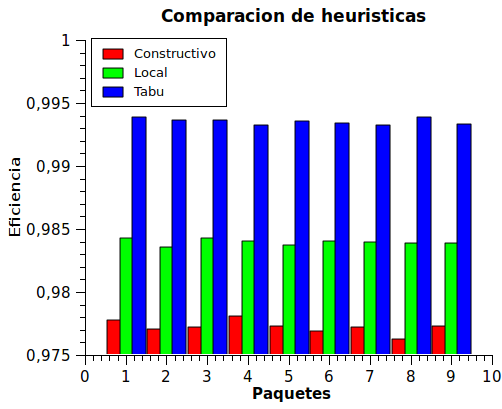
\includegraphics[width=0.7\textwidth]{graficos/combo1.png} 
\caption{Gráfico 1}
\end{figure}


Dado el gr\'afico presentado se pueden hacer varias observaciones:
\begin{itemize}
\item Las heur\'isticas muestran resultados esperados: En primer lugar, con la eficacia m\'as baja se encuentra la heur\'istica constructiva (Se destaca que igualmente el comportamiento es muy bueno, superando el 97,5 porciento de cl\'ausulas satisfechas en promedio). En segundo lugar, se encuentra la b\'usqueda local, lo cual es natural dado que la misma empieza desde la soluci\'on provista por la constructiva y luego la mejora. Por \'ultimo, se puede ver que la metaheur\'istica de b\'usqueda tab\'u es la m\'as eficiente de la tres, dando un salto de calidad importante llegando casi al 99,5 porciento de cl\'ausulas satisfechas en promedio en todos los paquetes.
\item Las 3 heur\'isticas poseen un comportamiento porcentual parecido en los 9 paquetes, mostrando que la eficacia parece depender intrinsecamente de las elecciones hechas por las rutinas, y no por otros factores como la cantidad de variables o de cl\'ausulas.
\end{itemize}


A continuaci\'on se muestra el an\'alisis de los tiempos de ejecuci\'on de cada una de las heur\'isticas para estos paquetes de casos de prueba.


\begin{figure}[H]
\centering
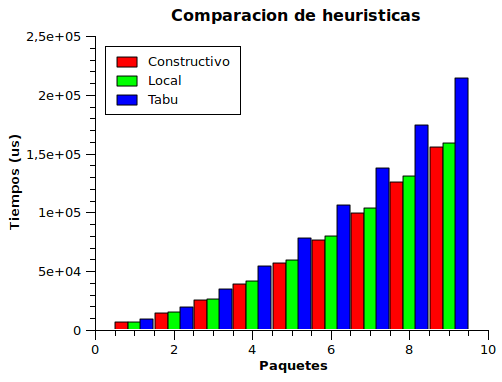
\includegraphics[width=0.7\textwidth]{graficos/combo1Tiempos.png} 
\caption{Gráfico 2}
\end{figure}



Como se puede ver en la figura 2, la heur\'istica constructiva es la que menos tiempo de ejecuci\'on toma lo cual concuerda con lo esperado ya que las otras dos heur\'isticas comienzan con la soluci\'on de la constructiva. Luego, se encuentra la heur\'istica de b\'usqueda local y por \'ultimo, con mayor tiempo de ejecuci\'on, se encuentra la b\'usqueda tab\'u.

Cabe destacar que la diferencia en los tiempos de ejecuci\'on entre la heur\'istica constructiva y la b\'usqueda local no es muy grande, mientras que la diferencia con tab\'u si es bastante mayor. Esto indicar\'ia que si bien la b\'usqueda local mejora los resultados de la heur\'istica constructiva(como se ve en el gr\'afico 1), no toma mucho tiempo en hacerlo ya que r\'apidamente cae en un m\'aximo local. Por otro lado, la b\'usqueda tab\'u si toma un tiempo mayor, porque aunque caiga en m\'aximos locales, sigue buscando dada su naturaleza, es esta brecha en el tiempo de ejecuci\'on la que explica la clara diferencia en la eficacia de tab\'u al realizar una b\'usqueda m\'as exahustiva.

\bigskip

La eficacia superior que mostr\'o la b\'usqueda tab\'u, motiva la siguiente secci\'on de an\'alisis realizada para hacer m\'as hincapie en la eficacia de esta metaheur\'istica, as\'i como la de su modificaci\'on implementada.

\subsection*{An\'alisis comparativos de variaciones de par\'ametros en b\'usqueda tab\'u y tab\'u modificada}
\addcontentsline{toc}{subsection}{An\'alisis comparativos de variaciones de par\'ametros en b\'usqueda tab\'u y tab\'u modificada}

En primer lugar, se destaca que el an\'alisis de todos los casos siguientes se realiz\'o de la misma manera que en la secci\'on anterior; es decir, se utilizaron los mismos nueve paquetes de casos de prueba, y para resumir el desempe\~{n}o se utiliz\'o el mismo n\'umero de eficacia presentado anteriormente.

Una vez realizadas dichas consideraciones, se proceder\'a a realizar el an\'alisis pertinente. Dicho an\'alisis esta basado en las siguientes propiedades: 

La metaheur\'istica de b\'usqueda tab\'u posee tres par\'ametros que son modificables, los mismos son: Longitud de la lista tab\'u, Cantidad m\'axima de iteraciones y Cantidad m\'axima de iteraciones entre \'optimos. Es por esto que lo que se har\'a es analizar como var\'ia la eficacia y el tiempo de ejecuci\'on de la b\'usqueda tab\'u al modificar estos par\'ametros.

Por otro lado, la b\'usqueda tab\'u modificada presenta un par\'ametro m\'as que es la cantidad de asignaciones con las que se trabaja, por lo que el \'ultimo an\'alisis presentado sera pertinente a la variaci\'on de este par\'ametro.

\bigskip

\subsubsection*{Longitud de la lista tab\'u}

En primer lugar, se comenzar\'a el an\'alisis fijando los par\'ametros de cantidad de iteraciones, y se modificar\'a la longitud de la lista tab\'u. La longitud de la lista tab\'u se vari\'o entre v/3 y v/9, mientras que la cantidad m\'axima de iteraciones queda fija en 3*v y la cantidad m\'axima de iteraciones entre \'optimos queda fija en v/2

A continuaci\'on, se puede ver el gr\'afico de la eficacia en funci\'on de cada paquete. 


\begin{figure}[H]
\centering
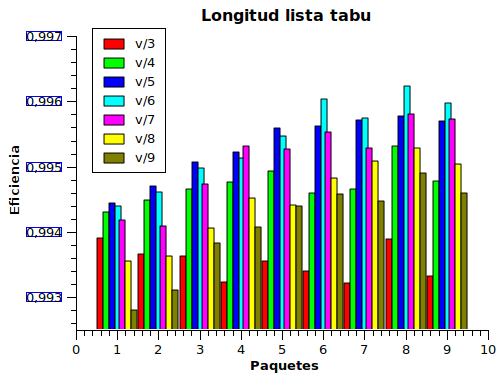
\includegraphics[width=0.7\textwidth]{graficos/combo3.png} 
\caption{Gráfico 3}
\end{figure}

Dado el gr\'afico de la figura 3, se puede ver como var\'ia la eficacia de la b\'usqueda tab\'u dependiendo de la longitud de la lista. La conclusi\'on principal que se desprende de la visualizaci\'on del gr\'afico es que las franjas centrales se encuentran por encima de las franjas laterelas. Es decir, parecer\'ia ser que la metaheur\'istica funciona de mejor manera cuando la longitud de la lista se encuentra entre v/5, v/6 y v/7 y comienza a bajar su eficacia a medida que la longitud se aleja de estos valores.

En el gr\'afico se denota que en los primeros paquetes v/5 parece ser la longitud m\'as eficaz, mientras que en los \'ultimos paquetes es v/6 la que aparece por encima de las dem\'as. v/7 solo es la m\'as eficiente en el 4to paquete, pero en todos los demas se encuentra cerca del m\'aximo.

Es importante destacar que si bien se encuentran fluctuaciones y tendencias, todas las longitudes propuestas se encuentran en un margen muy chico, resultando todas muy eficientes.

Por \'ultimo, se destaca que las tendencias vistas sobre la mejor longitud para la lista tab\'u se condice con los resultados encontrados en la bibliograf\'ia.\footnote{Ver cita bibliogr\'afica 1}

\bigskip

A continuaci\'on, se presenta el gr\'afico de los tiempos de ejecuci\'on de la metaheur\'istica al cambiar la longitud de la lista tab\'u.

\begin{figure}[H]
\centering
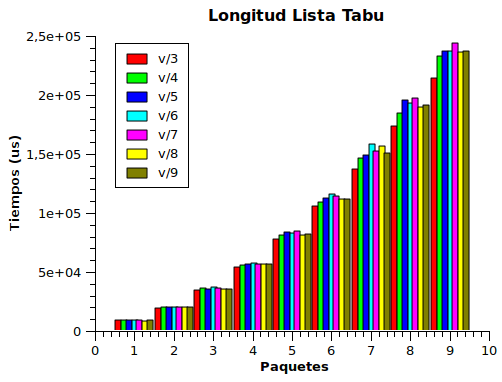
\includegraphics[width=0.7\textwidth]{graficos/combo3Tiempos.png} 
\caption{Gráfico 4}
\end{figure}



Como se puede ver en el gr\'afico, no hay grandes fluctuaciones entre los tiempos de ejecuci\'on y se encuentra ninguna tendencia muy definida. Esto se debe a que mirar si una asignaci\'on se encuentra restringidad por la lista tab\'u es O(1), entonces no es importante cu\'al es la longitud de la misma, ya que no tiene impacto sobre el tiempo de ejecuci\'on.

\subsubsection*{Cantidad m\'axima de iteraciones}

En esta parte se analizar\'a como var\'ia la eficiencia y el tiempo de ejecuci\'on de la metaheur\'istica, al cambiar el valor de la cantidad m\'axima de iteraciones permitidas. Por otro lado, la longitud de la lista tab\'u queda fija en v/3, mientras que la cantidad m\'axima de iteraciones entre \'optimos queda fija en v/2.

A continuaci\'on, se presenta el gr\'afico de eficiencia en funci\'on de los paquetes de casos de prueba.

\begin{figure}[H]
\centering
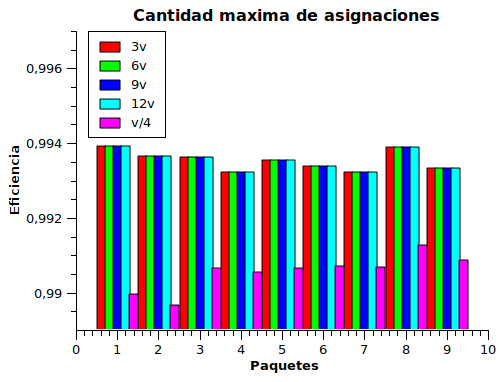
\includegraphics[width=0.7\textwidth]{graficos/combo4.png} 
\caption{Gráfico 5}
\end{figure}


En el gr\'afico presentado anteriormente se pueden denotar dos cosas importantes:
\begin{itemize}
\item En primer lugar se puede ver que cuando el par\'ametro toma los valores 3*v, 6*v, 9*v y 12*v todas las eficiencias dan exactamente el mismo resultado. Esto se cree que se debe a que cuando el par\'ametro toma estos valores se hace obsoleto, ya que lo que debe estar suceciendo es que la cantidad m\'axima de iteraciones entre \'optimos siempre poner una cota menor y nunca se llega a la cota que aqu\'i esta variando. 
\item Por otro lado, se puede ver que cuando se baja mucho el par\'ametro (v/4), la meteheur\'istica se degrada considerablemente ya que se impone una cota muy baja para la cantidad total de iteraciones.
\end{itemize}


Luego de ver como se comporta la b\'usqueda tab\'u al cambiar el par\'ametro del m\'aximos de iteraciones, se presenta como se comporta la misma pero ahora en cuanto a tiempos de ejecuci\'on.

A continuaci\'on se puede ver el gr\'afico de tiempo de ejecuci\'on en funci\'on de los paquetes.

\begin{figure}[H]
\centering
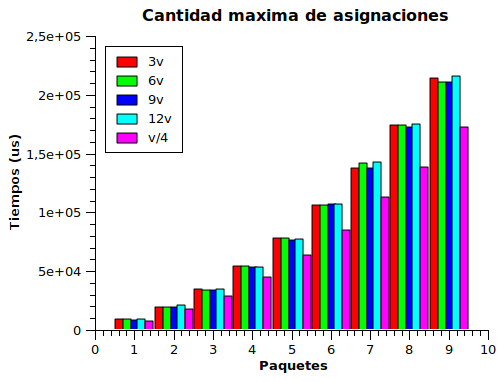
\includegraphics[width=0.7\textwidth]{graficos/combo4Tiempos.png} 
\caption{Gráfico 6}
\end{figure}

Lo que se puede ver en el gr\'afico anterior, es como los tiempos de ejecuci\'on se condicen con los resultados de eficiencia obtenidos. Los valores correspondientes a 3*v, 6*v, 9*v y 12*v tardan todos el mismo tiempo, reforzando lo augurado anteriormente; es decir, que nunca se llega a esta cota si no que la cota de cantidad m\'axima de operaciones entre \'optimos corta primero. Por otro lado, los valores correspondientes a v/4 son claramente menor a los dem\'as mostrando el claro \emph{tradeoff} natural, los tiempos de ejecuci\'on son mejores, pero al costo de tener menos eficiencia.


\subsubsection*{Cantidad m\'axima de iteraciones entre \'optimos}

En esta parte se ver\'a como var\'ia la eficiencia y los tiempos de ejecuci\'on cuando se modifica la cantidad m\'axima de iteraciones entre \'optimos, mientras que la longitud de la lista tab\'u queda fija en v/3 y la cantidad m\'axima de iteraciones queda fija en 3*v

A continuaci\'on se presenta el gr\'afico de eficiencia en funci\'on de los paquetes de casos de prueba:

\begin{figure}[H]
\centering
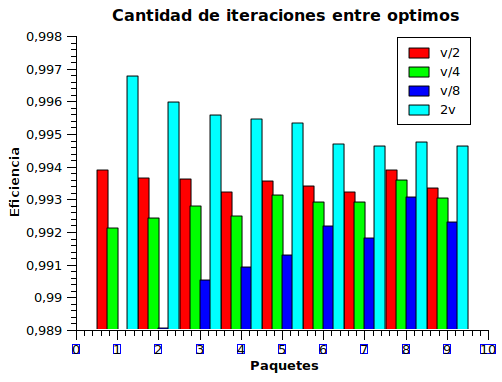
\includegraphics[width=0.7\textwidth]{graficos/combo5.png} 
\caption{Gráfico 7}
\end{figure}

Lo que se puede denotar en el gr\'afico anterior es una conclusi\'on bastante natural. A medida que se va achicando la cota, y cada vez se permite menos iteraciones, la eficiencia va bajando ya que la rutina va teniendo menos iteraciones para encontrar los mejores valores. En el momento que la cota se sube considerablemente a 2*v, la eficiencia crece.

A continuaci\'on se presenta el gr\'afico de los tiempos de ejecuci\'on para esta variaci\'on presentada.

\begin{figure}[H]
\centering
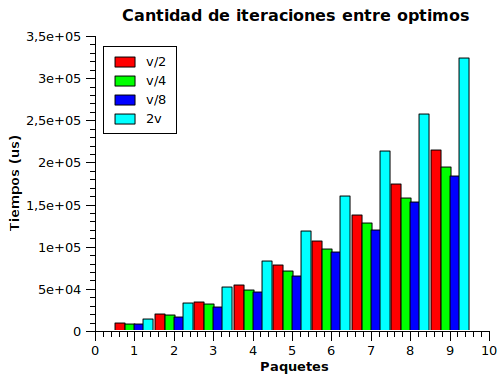
\includegraphics[width=0.7\textwidth]{graficos/combo5Tiempos.png} 
\caption{Gráfico 8}
\end{figure}

En este gr\'afico se puede ver como los tiempos de ejecuci\'on se condice perfectamente con los resultados obtenidos en la eficiencia. A medida que la cota baja, tambi\'en baja el tiempo de ejecuci\'on; y cuando la cota sube, el tiempo de ejecuci\'on tambi\'en lo hace. Al igual que en la secci\'on anterior, se puede como al variar este par\'ametro los tiempos de ejecuci\'on son peores si la eficiencia es mejor y viceversa.


\bigskip

Como conclusiones generales de la tres variaciones de par\'ametros hechas anteriormente se pueden destacar:

\begin{itemize}
\item La metaheur\'istica tiende a comportarse de manera m\'as eficiente cuando la longitud de la lista tab\'u se encuentra cerca de v/5 y v/6.
\item En cuanto a los otros dos par\'amtros se puede ver que ambos par\'ametros terminan siendo una soluci\'on de compromiso. Es decir, si se relajan mucho y las cotas son muy altas la eficiencia aumenta pero tambi\'en aumenta el tiempo de ejecuci\'on; mientras que si las cotas son bajas el tiempo de ejecuci\'on baja al costo de tener una menor eficiencia. 
\end{itemize}

\subsubsection*{An\'alisis Tab\'u modificado}

En el momento de an\'alisis del comportamiento de la metaheur\'istica de tab\'u modificada es importante notar que la misma posee 4 par\'ametros, los 3 primeros son los mismos que en tab\'u. El nuevo par\'ametro es la cantidad de asignaciones con la que se va a trabajar. Es por esto que para an\'alisar este tab\'u modificado se van a fijar los 3 par\'ametros que comparte con la b\'usqueda tab\'u original y se ir\'a variando la cantidad de asignaciones. 

En este an\'alisis los par\'ametros ser\'an fijados de la sigueinte manera: La longitud de la lista tab\'u ser\'a v/5, la cantidad m\'axima de iteraciones ser\'a v y la cantidad m\'axima de iteraciones entre \'optimos ser\'a v/2.

Por otro lado, la cantidad de asignaciones ser\'an 1, 2, 5, 10 y 50. Es importante destacar que cuando la cantidad de asignaciones es 1, esta b\'usqueda es la misma que la tab\'u original. Esta ser\'a la manera para poder comparar el comportamiento de la b\'usqueda tab\'u modificada con la b\'usqueda tab\'u original.


A continuaci\'on se presenta el gr\'afico de eficiencia en funci\'on de los paquetes de casos de prueba:



\begin{figure}[H]
\centering
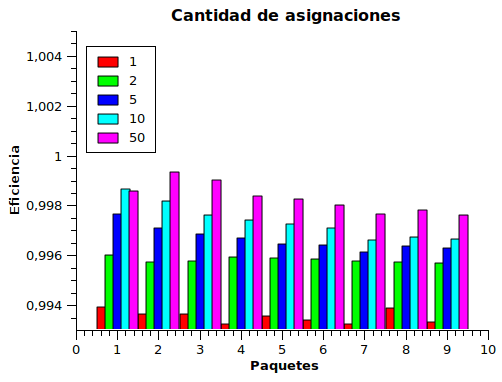
\includegraphics[width=0.7\textwidth]{graficos/combo2.png} 
\caption{Gráfico 9}
\end{figure}


Luego de presentar el anterior gr\'afico se puede concluir en que:

\begin{itemize}
\item La b\'usqueda tab\'u modificada presenta mejores resultados que la b\'usqueda tab\'u original.
\item A medida que se aumentan la cantidad de asignaciones el desempe\~{n}o mejora claramente (excepto en el primer paquete), llevando la eficiencia a niveles muy altos llegando a sobrepasar el 99,9 porciento de cl\'ausulas satisfechas.
\item Si bien cuando las asignaciones suben la eficiencia tambi\'en lo hace, se puede visualizar que a medida que las cl\'ausulas y las variables totales crecen la eficiencia tiende a decrecer. Se cree que a medida que crece la cantidad de variables, la cantidad de asignaciones va quedando chica en relaci\'on a la cantidad total de asignaciones que existe que crece exponencialmente.
\item Si bien lo mejor parece ser seguir incrementando la cantidad de asignaciones, es l\'ogico creer que esto tendra un impacto en el tiempo de ejecuci\'on que impondra restricciones.
\end{itemize}


A continuaci\'on se presenta el gr\'afico de tiempos de ejecuci\'on al variar la cantidad de asignaciones:

\begin{figure}[H]
\centering
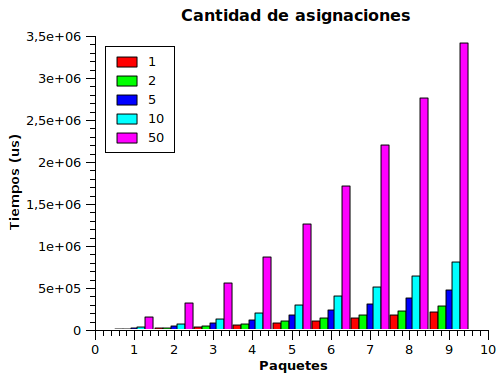
\includegraphics[width=0.7\textwidth]{graficos/combo2Tiempos.png} 
\caption{Gráfico 10}
\end{figure}


A partir del gr\'afico anterior se puede ver claramente como la conjetura realizada anteriormente parece plasmarse. Es decir, si bien subir la cantidad de asignaciones hace crecer la eficiencia de los resultados, tambi\'en crece de manera abrupta el tiempo de ejecuci\'on requerido. 

Es por esto que se puede concluir algo similar a lo concluido anteriormente con los par\'ametros de cantidad de iteraciones. Si bien variarlos puede traer mejores resultados, tambi\'en tiene fuerte impacto en el tiempo de ejecuci\'on. 

Cabe destacar como conclusi\'on general de la b\'usqueda tab\'u modificada que esta gener\'a resultados muy eficientes, muy cercanos a la soluci\'on exacta en la mayor\'ia de los casos.



\section*{Conclusiones}
\addcontentsline{toc}{section}{Conclusiones}

Luego de realizar los an\'alisis de resultados de todos los algoritmos y heur\'isticas implementadas se puede concluir varios puntos sobre este trabajo y tambi\'en sobre mejoras que se podr\'ian realizar en ampliaciones futuras de \'este:

\begin{itemize}
\item La implementaci\'on de algoritmos exactos para este tipo de problemas no es viable ya que al ir creciendo el tama\~{n}o de las instacias de prueba, los tiempos de ejecuci\'on resultan inmanejables, siempre y cuando los mismos sean exponenciales. Aun as\'i para trabajos futuros podr\'ia ser importante tratar de mejorar el algoritmo de backtraking, tomando como punto de partida las podas realizadas en este trabajo, pero generando otros criterios que ayuden a podar las ramas del arbol, para poder ahorrar tiempo de ejecuci\'on.
\item Es importante poder generar otros tipos de filtros para todos los algoritmos y heur\'isticas propuestas. Sin embargo, en el caso del filtro de componentes conexas se pudo ver que este trabajo no fue fruct\'ifero, por lo que su implementaci\'on fue dejada en un segundo plano.
\item Para trabajos futuros, se podria indagar m\'as no solamente en las decisiones que las heur\'isticas toman sino tambi\'en en las estructuras utilizadas para implementarlas, una mejora considerable en estas podr\'ia ser un punto importante a tener en cuenta.
\item La meteheur\'istica de b\'usqueda tab\'u y posterior modificaci\'on presentaron resultados realmente eficientes, llegando a sobrepasar el 99,5 porciento de cl\'ausulas satisfechas en todos los casos. Es por esto que se cree que la principal conclusi\'on de este trabajo es que en trabajos futuros, con mayor tiempo de desarrollo, se deber\'ia ahondar m\'as en estas heur\'isticas, buscando nuevas modificaciones que resulten eficientes. 
\item En \'ultimo lugar, cabe destacar que no se pudo contrastar los resultados con las complejidades temporales calculadas durante el trabajo. Esto se debi\'o a que en los casos de prueba disponibles la cantidad cl\'ausulas y variables no guardan una relaci\'on que luego se pueda constratar con la complejidad. Podr\'ia ser un buen punto para ampliaciones futuras el hecho de generar casos de prueba especialmente dedicados a verificar empiricamente si la complejidad te\'orica calculada es correcta.
\end{itemize}

\newpage
\section*{Ap\'endice 1: Bibliograf\'ia}
\addcontentsline{toc}{section}{Ap\'endice 1: Bibliografia}

\begin{itemize}
\item ``Algorithms for the Maximum Satiasfiability Problem", Pierre Hansen, USA. 
\item  ``A user's guide to tabu search", Fred Glover, USA.
\item ``Tabu search", Alain Hertz, Lausane.
\item http://wiki.org.es/.
\end{itemize}

\newpage
\section*{Ap\'endice 2: Instrucciones para utilizar benchmarks.cpp}
\addcontentsline{toc}{section}{Instrucciones para utilizar benchmarks.cpp}
A continuaci\'on se explica como utilizar el archivo benchmarks.cpp para correr muchas pruebas en formato cnf.

Cabe destacar que este archivo se encuentra pensado para funcionar en un sistema operativo tipo Linux.

\begin{enumerate}
\item Crear una carpeta nueva, el path a esa carpeta va a ser $PATH/carpeta_nueva$. Donde PATH puede ser cualquier directorio.
\item Crear $PATH/carpeta_nueva/output$. Es Aqu\'i donde se copiar\'an los resultados finales.
\item Mover a $PATH/carpeta_nueva$ los archivos $mostrar_satisfechos.cpp$ y dimacs2algo.cpp. Es importante realizar esto, ya que dimacs2algo.cpp es el conversor de formato cnf al formato requerido para este trabajo.
\item Compilar el cpp del algoritmo que se quiera correr con el flag -DTIEMPOS (en el caso que se quiera obtener los tiempos de corrida) y copiar el ejecutable a $PATH/carpeta_nueva$
\item Poner en $PATH/carpeta_nueva$ archivos de formato cnf bajados de www.satlib.com. Asegurarse de copiar estos archivos en carpetas $PATH/carpeta_nueva/pruebas_xclausulas_yVariables$ y no en cualquier otro path.
\item Compilar benchmarks.cpp, copiar su ejecutable a $PATH/carpeta_nueva$.
\item Correrlo ./ Ejecutablebenchmark  ejecutableaprobar nombredelarchivooutput nombredearchivodetiempos
\end{enumerate}


\end{document}
